\documentclass[11pt, conference, onecolumn]{IEEEtran}
\IEEEoverridecommandlockouts
% The preceding line is only needed to identify funding in the first footnote. If that is unneeded, please comment it out.

\usepackage{cite}
\usepackage{amsmath,amssymb,amsfonts}
\usepackage{algorithmic}
\usepackage{graphicx}
\usepackage{textcomp}
\usepackage{xcolor}
\usepackage{multicol}
\usepackage{float}

\newcommand{\rom}[1]{\uppercase\expandafter{\romannumeral #1\relax}}
\def\BibTeX{{\rm B\kern-.05em{\sc i\kern-.025em b}\kern-.08em
    T\kern-.1667em\lower.7ex\hbox{E}\kern-.125emX}}
%\begin{document}
%\title{Start Gap Wear Levelling for Phase Change Memory\\}
\author{\IEEEauthorblockN{Masih Ahmed}
\IEEEauthorblockA{\textit{CSE \rom{2} year} \\
\textit{IIT Roorkee}\\
18117056\\
mahmed@cs.iitr.ac.in}\\
%\and
\IEEEauthorblockN {Suraaj K S}
\IEEEauthorblockA{\textit{CSE \rom{2} year} \\
\textit{IIT Roorkee}\\
18117106\\
skanniwadi@cs.iitr.ac.in}
\and
\IEEEauthorblockN{ Divyanshu Setia}
\IEEEauthorblockA{\textit{CSE \rom{2} year} \\
\textit{IIT Roorkee}\\
18114020\\
dsetia@cs.iitr.ac.in}\\
%\and
\IEEEauthorblockN{Rishi Chordia}
\IEEEauthorblockA{\textit{CSE \rom{2} year} \\
\textit{IIT Roorkee}\\
18118052\\
rchordia@cs.iitr.ac.in}
\and
\IEEEauthorblockN{Vanshika Bhargava}
\IEEEauthorblockA{\textit{ECE \rom{2} year} \\
\textit{IIT Roorkee}\\
18117112\\
vbhargava@ec.iitr.ac.in}\\
%\and
\IEEEauthorblockN{Kshitij Srikant}
\IEEEauthorblockA{\textit{ECE \rom{2} year} \\
\textit{IIT Roorkee}\\
18117047\\
ksrikant@ec.iitr.ac.in}
\and 
\IEEEauthorblockN{Burri Vishnu}
\IEEEauthorblockA{\textit{ECE \rom{2} year} \\
\textit{IIT Roorkee}\\
18116024\\
breddy3@ec.iitr.ac.in}
}
\title{Start Gap Wear Levelling for Phase Change Memory\\}
\begin{document}
\maketitle
~\\
\begin{abstract}
Modern main memory present today is heavily based on DRAM,namely SDRAM. However, modern memory consisting
entirely of DRAM is already hitting power and cost limits.
Exploiting emerging memory technologies, such as Phase-Change
Memory (PCM) and Flash, has become crucial to build larger capacity memory systems in the future while remaining within the
overall system cost and power budgets.\\
\newline
Phase Change Memory (PCM) is an emerging memory technology that can increase main memory capacity in a cost-effective and
power-efficient manner. However, PCM cells can endure only a
maximum of 10\textsuperscript{7 }- 10\textsuperscript{8} writes, making a PCM based system have
a lifetime of only a few years under ideal conditions. Furthermore,
we show that non-uniformity in writes to different cells reduces the
achievable lifetime of PCM system by 20x. Writes to PCM cells
can be made uniform with Wear-Leveling. Unfortunately, existing
wear-leveling techniques require large storage tables and indirection, resulting in significant area and latency overheads. \\
\\We implement Start-Gap, an effective wear-leveling
technique that uses only two registers. By combining Start-Gap
with simple address-space serialisation techniques we show that
the achievable lifetime of the PCM storage cell.\\
\end{abstract}
\section{Modern memory hierarchy}
Modern systems featuring deep memory hierarchies and many parallel processing units, breaking large computations into smaller operations is essential to achieving good performance because it exposes parallelism and results in efficient execution on datasets stored local to processing elements. The level of heirarchy is found in  essentially all
 Common examples of this optimization technique include blocking to increase cache locality and problem decomposition to minimize network communication in MPI programs for clusters \\
\\ There are four major storage levels
\begin{enumerate}
  \item Internal – Processor registers and cache.
  \item Main – the system RAM and controller cards.
  \item On-line mass storage – Secondary storage.
  \item Off-line bulk storage – Tertiary and Off-line storage.
\end{enumerate}
The memory hierarchy of an Intel Haswell Mobile processor circa 2013 is:
\begin{itemize}
	\item Processor registers – the fastest possible access (usually 1 CPU cycle). A few thousand bytes in size.
	\item Cache
		\begin{itemize}
			\item Level 0 (L0) Micro operations cache - 6 KB  in size
        			\item Level 1 (L1) Instruction cache - 128 KB in size
        			\item Level 1 (L1) Data cache - 128 KB in size. Best access speed is around 700 GB/second
        			\item Level 2 (L2) Instruction and data (shared) - 1 MB in size. Best access speed is around 200 GB/second
        			\item Level 3 (L3) Shared cache - 6 MB in size. Best access speed is around 100 GB/second
        			\item Level 4 (L4) Shared cache - 128 MB in size. Best access speed is around 40 GB/second
		\end{itemize}
\begin{figure}
		\begin{center}
		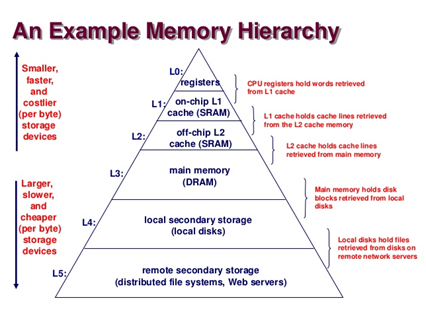
\includegraphics[width=0.8\textwidth]{memory.png}
		\caption {Memory hierarchy}
		\end{center}	
	\end{figure}
	\item Main memory (Primary storage) - Gigabytes in size. Best access speed is around 10 GB/second. In the case of a NUMA machine, access times may not be uniform.
	\item Disk storage (Secondary storage) - Terabytes in size. As of 2017, best access speed is from a consumer solid state drive is about 2000 MB/second.
	\item Nearline storage (Tertiary storage) - Up to exabytes in size. As of 2013, best access speed is about 160 MB/second.
\end{itemize}
\section{DRAM Heirarchy}
The rank of a DRAM module is the highest level of organization within a DIMM. Below that, each chip is organized into a number of banks and memory arrays containing rows and columns. Figure shows a DRAM chip with four banks. \\
\begin{figure}
		\begin{center}
		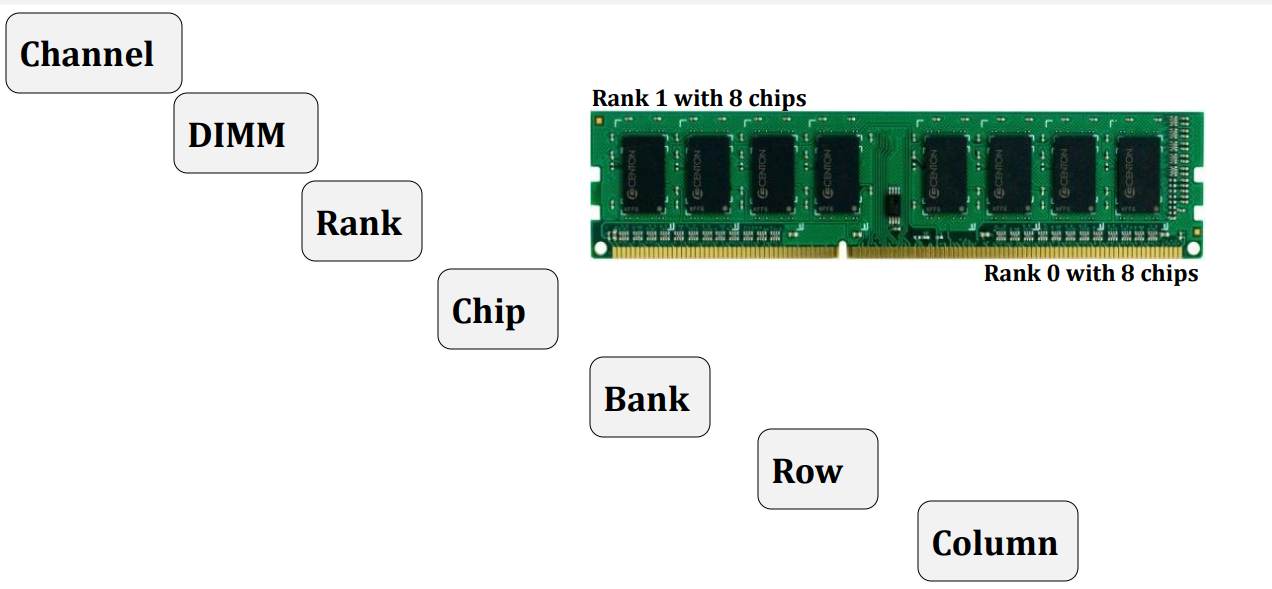
\includegraphics[width=0.8\textwidth]{dramorg.png}
		\caption {DRAM organisation in memory}
		\end{center}	
	\end{figure}\\The rank of a DRAM is a set of separately addressable DRAM chips. Each DRAM chip is further organized into a number of banks that contain a set of memory arrays. The number of memory arrays per bank is equal to the size of the output width. Therefore, in a x4 
DRAM chip, the internal banks would each have four memory arrays. Figure shows an example of a single x4 bank.\\
\\The grey section is the memory array designed as a grid of rows and columns. A set of decoders are used to access the rows and columns, selecting a single intersection within the memory array. It is at this intersection that a small capacitor stores a charge representing the data being accessed.\\
\begin{figure}[!tbp]
  \centering
  \begin{minipage}[b]{0.4\textwidth}
    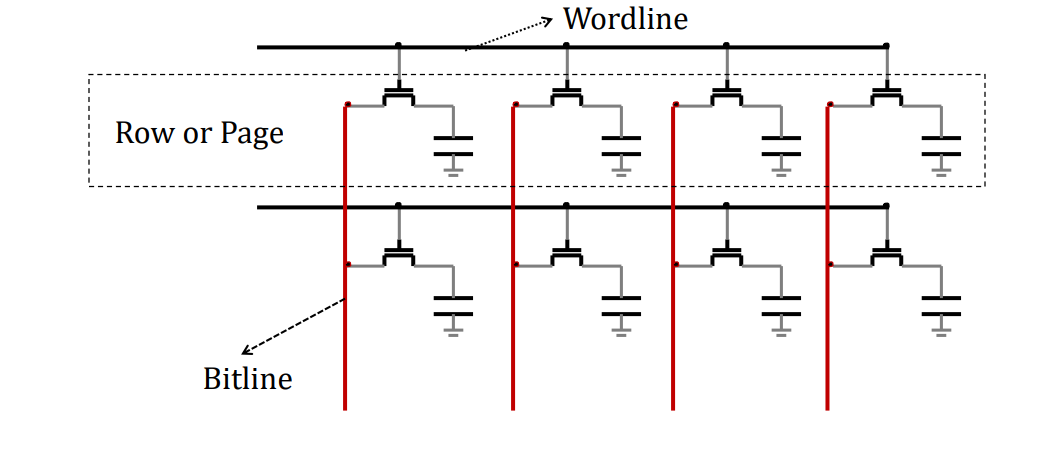
\includegraphics[width=\textwidth]{dramcell.png}
    \caption{DRAM Cell}
  \end{minipage}
  \hfill
  \begin{minipage}[b]{0.4\textwidth}
    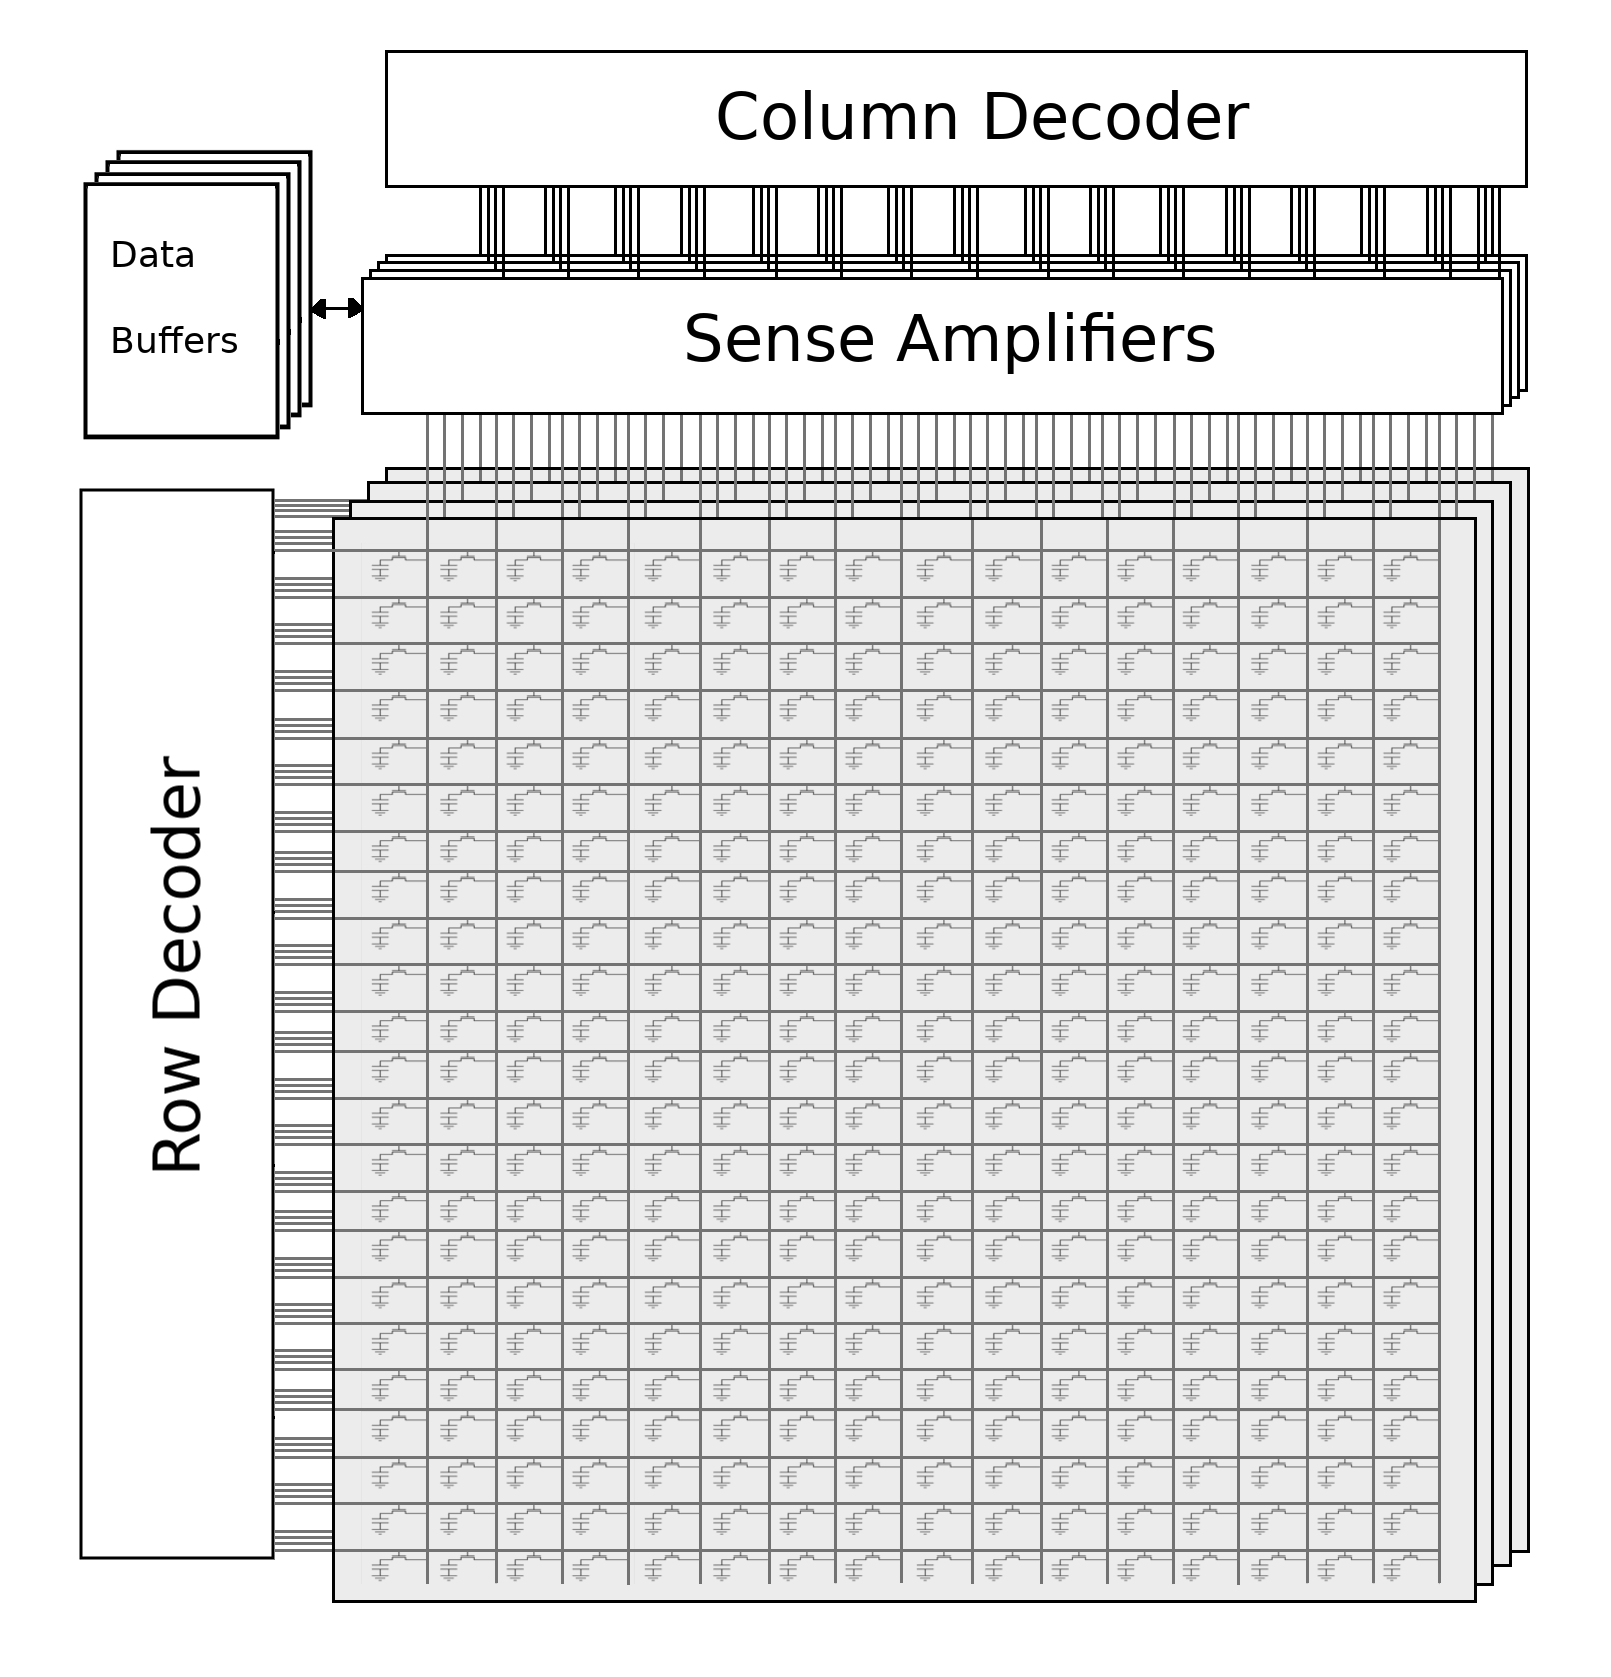
\includegraphics[width=\textwidth]{bank.png}
    \caption{DRAM bank}
  \end{minipage}
\end{figure}
\\Sense amplifiers perform precharge operations on capacitors and generate logic-level outputs for a number of data buffers that store the data until it can be retrieved by a memory controller or CPU.\\
\\DRAM is extremely common in personal computers and is a basic component that any computer needs to work properly. DRAM works by using the presence or absence of charge on a capacitor to store data. Since a single DRAM cell is composed of only two
components - a transistor and a capacitor - DRAM can be made in high densities, and it is inexpensive compared to other types of memory.\cite{b1}
\\
\\

\section{The need for new memory technologies - DRAM scaling problems}
Technology scaling of DRAM cells has enabled higher capacity memory for the last few decades. Unfortunately, DRAM cells become vulnerable to failure as they scale down to a smaller size. Enabling high-performance, energy-efficient, scalable memory systems without sacrificing the reliability is a major research challenge.\\ DRAM scaling issues are cause due to increasing cell-to-cell interference along with decreasing capacitor reliability.
\\Three fundamental ways to enable DRAM scaling are described below. First, we can enable scaling by letting the manufacturers build smaller cells without providing any strict reliability guarantee. Manufacturers ship DRAMs without fully ensuring correct operation, and the system being responsible for detecting and mitigating DRAM failures while operating in the field. However, designing such a system is difficult due to intermittent DRAM failures. A system design, capable of providing reliability guarantees even in the presence of intermittent failures. Second, tolerating failures in the application can improve DRAM scalability. The fundamental challenge of such a system is how to assure, verify, and quantify the quality of the results.A system that limits the impact of memory failures such that it is possible to statically determine the worst-case results from the maximum possible error in the input. Third, we can enable high-capacity memory leveraging the emerging non-volatile memory technologies that are predicted to be more scalable.
\\
\\
\section{Phase change memory}
One of the potential successors of DRAM is a class of memory called Resistive Random-access memory, or RRAM for short. RRAM is based on a new type of semiconductor material that forms digital zeros and ones by resisting or permitting the flow of electrons. RRAM has the potential to do things that aren’t possible with silicon: for instance, being layered on top of computer transistors in new three-dimensional, high-rise chips that would be faster and more energy efficient than current electronics, which is ideal for smartphones and other mobile devices where energy efficiency is a vital feature.\\
\\RRAM materials are insulators, which normally do not allow electricity to flow. But under certain circumstances, insulators can be induced to let electrons flow. Jolting RRAM materials with an electric field causes a pathway to form that permitted electron flows. This pathway is called a filament. To break the filament, researchers apply another jolt and the material becomes an insulator again. So each jolt switched the RRAM from zero to one or back, which is what makes the material useful for data storage.\\
\\The PCM device is essentially a resistor of a thin-film chalcogenide material, usually a Ge–Sb–Te alloy with a low-field resistance that changes by orders of magnitudes, depending on the phase state of the material in the active region (i.e., crystalline or amorphous). In memory operation, cell readout is performed at low bias by sensing the resistance value. PCM technology has the potential to provide inexpensive, high-speed, high-density, high-volume non-volatile storage on an unprecedented scale. Because it is much closer in speed to dynamic RAM (DRAM), phase change memory technology is ideal for both non-volatile dual in-line memory modules (NVDIMMs) and non-volatile memory express (NVMe) solid state drives (SSDs).\\
\\In order to increase the main memory capacity and increase the performance efficiency, it is necessary to use PCM or Flash along with DRAM. Flash is about 200x slower than DRAM and can endure a maximum of only 104 − 105 writes, which makes it unsuitable for main memory. PCM, on the other hand, is only 2x-4x slower than DRAM and can provide up to 4x more density than DRAM.\cite{b2}
\\
\\
\section{Write Endurance problem with PCM}
 Phase Change Memory (PCM) has emerged as a promising candidate for building the future main memory systems. However, the limited write endurance is one of the major obstacles for PCM to be practically applied. Traditional wear-leveling techniques try to uniformly balance the write traffics under both general applications and malicious attacks to enhance the PCM lifetime. However, these techniques fail to consider the endurance variation in PCM chips, and result in severe lifespan degradation since uniform write distribution leads to the weakest cell to be worn out much earlier. Nonetheless, it has a well-known problem that is the limited number of writes to storage cells. Thus, it is important to use certain techniques to boost PCM's lifetime. \\
\\One such technique is wear levelling method, it is used to create some sort of uniformity to improve performance efficiency. The storage and latency overhead of the indirection table in table based wear levelling can be eliminated if instead an algebraic mapping of logical address to physical address is used. Start-Gap wear levelling that uses an algebraic mapping between logical addresses and physical addresses, and avoids tracking per line write counts. Start-Gap performs wear levelling by periodically moving each line to its neighbouring location, regardless of the write traffic to the line. It consists of two registers: Start and Gap, and an extra memory line Gap Line to facilitate data movement. Gap tracks the number of lines relocated in memory and Start keeps track of how many times all the lines in memory have been relocated.
\\
\\
\section{Wear levelling techniques}
Typically there is a significant non-uniformity in write traffic to memory lines. This causes the heavily written lines to fail much earlier than expected system lifetime. For the baseline system, this non-uniformity causes the actual lifetime to be 20x lower than lifetime achievable under ideal conditions. The lifetime of a PCM system can be improved by making writes uniform throughout the entire memory space. Wear leveling is a mechanism that tries to make the writes uniform by remapping heavily written lines to less frequently written lines. We implement a software version of a simple wear levelling technique, called \textit{Start Gap Wear Levelling}\cite{b3}.
\\
\\
\section{Start-Gap algorithm}
Figure 5(a) shows a memory system consisting of 16 lines (0-15). To implement Start-Gap, an extra line (GapLine) is added at
location with address 16. The 17 lines can be visualized as forming
a circular buffer. GapLine is a memory location that contains no
useful data. Two registers, Start and Gap are also added. Start
initially points to location 0, and Gap always points to the location
of the GapLine. To perform wear leveling, Gap is moved by 1
location once every ψ writes to memory. The move is accomplished
simply by copying the content of location of [Gap-1] to GapLine
and decrementing the Gap register. This is shown by movement of
Gap to line 15 in Figure 5(b). Similarly, after 8 movements of Gap
all the lines from 8-15 get shifted by 1, as indicated in Figure 5(c).\\
	\begin{figure}
		\begin{center}
		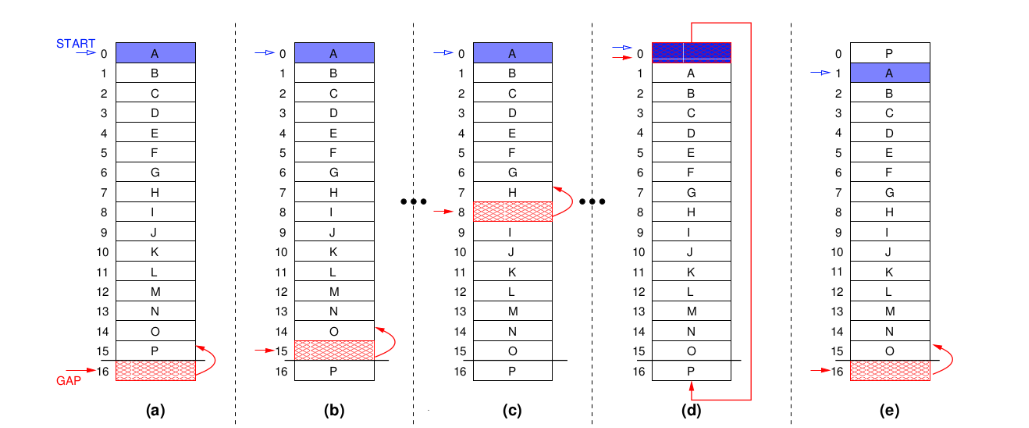
\includegraphics[width=20cm, height=10cm]{sga.png}
		\caption {Start-Gap wear leveling on a memory containing 16 lines.}
		\end{center}	
	\end{figure}
\begin{figure}[!tbp]
  \centering
  \begin{minipage}[b]{0.4\textwidth}
    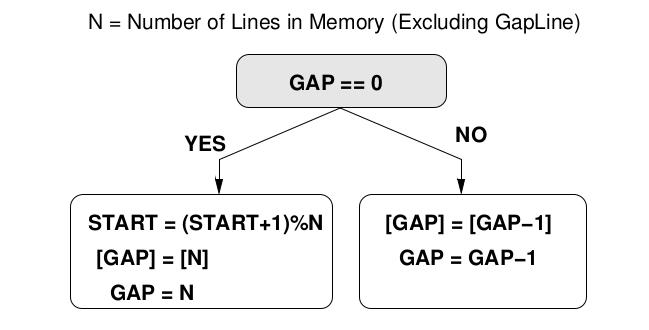
\includegraphics[width=\textwidth]{flow1.png}
    \caption{Flowchart for Gap Movement.}
  \end{minipage}
  \hfill
  \begin{minipage}[b]{0.4\textwidth}
    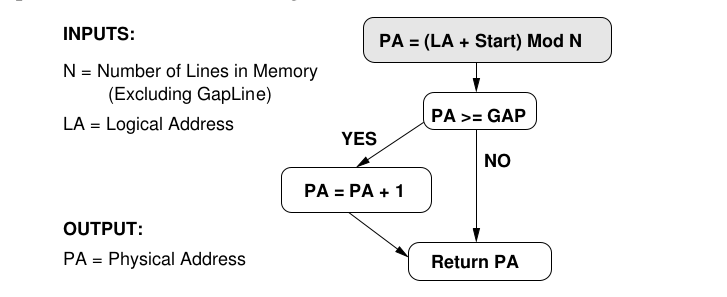
\includegraphics[width=\textwidth]{flow2.png}
    \caption{Mapping of Logical Address to Physical Address.}
  \end{minipage}
\end{figure}
~\\Figure 5(d) shows the case when Gap reaches location 0, and
Line 0 - Line 15 have each moved by 1 location. As with any
circular buffer, in the next movement, Gap is moved from location
0 to location 16 as shown in Figure 5(e). Note that Figure 5(e) is
similar to Figure 5(a) except that the contents of all lines (Line 0
to Line 15) have shifted by exactly 1 location, and hence the Start
register is incremented by 1. Every movement of Gap provides
wear leveling by remapping a line to its neighboring location. For
example, a heavily written line may get moved to a nearby read-
only line. To aid discussion, we define the terms Gap Movement
and Gap Rotation as follows: 
\\\textbf{Gap Movement:} This indicates movement of Gap by one, as
shown in Figure 5(a) to Figure 5(b). We perform Gap Movement
once every ψ writes to the main memory, where ψ is a parame-
ter that determines the wear leveling frequency. Gap register is
decremented at every Gap Movement. If Gap is 0, then in the next
movement it is set to N (the number of locations in memory).
\\\textbf{Gap Rotation:} This indicates all lines in the memory have per-
formed one Gap Movement for a given value of Start. The Start
register is incremented (modulo number of memory lines) on each
Gap Rotation. Thus, for a memory containing N lines, Gap Rota-
tion occurs once every (N + 1) Gap Movement. The flowchart for
Gap Movement (and Gap Rotation) is described in Figure 6.\\
\\The Gap and Start registers change continuously which changes
the mapping of logical to physical memory addresses. The mapping
is accomplished by making two observations: (1) In Figure 5(c) all
addresses more than or equal to Gap, are moved by 1 and all loca-
tion less than Gap remain unchanged. (2) When Start moves as in Figure 5(e) all locations have moved by 1, so the value of Start
must be added to the logical address to obtain physical address. The
mapping is captured by the pseudo-code shown in Figure 7, which
may be trivially implemented in hardware using few gates. If PA is
less than N then memory is accessed normally. If PA=N then the
spare line (Location 16 in Figure 5) is accessed.
\\
\\
\section{C Implementation of Start-Gap algorithm}
\begin{verbatim}
int translate(int logicalAddress)
{
	int physicalAddress = (logicalAddress + start) % (MEMSIZE-1);
	if(physicalAddress >= gap) return physicalAddress +1;
	else return physicalAddress;
}

void memAccess(int logicalAddress,int inp)
{
	writeCount ++;
	if(writeCount % phi != 0)
	{
		memory [translate(logicalAddress)] = inp;
		return;
	}
	

	if(gap != 0)
	{
		memory[gap] = memory[gap-1];
		gap--;
		memory [translate(logicalAddress)] = inp;
		return;
	}

	start = (start+1)%(MEMSIZE-1);
	memory[gap] = memory[MEMSIZE-1];
	gap = MEMSIZE-1;
	memory [translate(logicalAddress)] = inp;

}
\end{verbatim}
\section*{Acknowledgment}
We thank Dr. P Satish Kumar for his guidance in the project.
\\
\\
\begin{thebibliography}{00}



\bibitem{b1} Phoenix Corp, on "Integrated Circuit Engineering Corporation" - 7-1, "DRAM Technology"
\bibitem{b2}B. Lee, E. Ipek, O. Mutlu, and D. Burger. Architecting phase
change memory as a scalable dram alternative. In ISCA ’09:
Proceedings of the 36th annual international symposium on
Computer architecture, 2009.
\bibitem{b3} Moinuddin K. Qureshi, John Karidis, Michele Franceschini, Vijayalakshmi Srinivasan, Luis Lastras, Bulent Abali on "Enhancing Lifetime and Security of PCM-Based
Main Memory with Start-Gap Wear Leveling"
\end{thebibliography}
\vspace{12pt}

%\end{multicols}
\end{document}
